% Options for packages loaded elsewhere
\PassOptionsToPackage{unicode}{hyperref}
\PassOptionsToPackage{hyphens}{url}
%
\documentclass[
]{book}
\usepackage{amsmath,amssymb}
\usepackage{lmodern}
\usepackage{iftex}
\ifPDFTeX
  \usepackage[T1]{fontenc}
  \usepackage[utf8]{inputenc}
  \usepackage{textcomp} % provide euro and other symbols
\else % if luatex or xetex
  \usepackage{unicode-math}
  \defaultfontfeatures{Scale=MatchLowercase}
  \defaultfontfeatures[\rmfamily]{Ligatures=TeX,Scale=1}
\fi
% Use upquote if available, for straight quotes in verbatim environments
\IfFileExists{upquote.sty}{\usepackage{upquote}}{}
\IfFileExists{microtype.sty}{% use microtype if available
  \usepackage[]{microtype}
  \UseMicrotypeSet[protrusion]{basicmath} % disable protrusion for tt fonts
}{}
\makeatletter
\@ifundefined{KOMAClassName}{% if non-KOMA class
  \IfFileExists{parskip.sty}{%
    \usepackage{parskip}
  }{% else
    \setlength{\parindent}{0pt}
    \setlength{\parskip}{6pt plus 2pt minus 1pt}}
}{% if KOMA class
  \KOMAoptions{parskip=half}}
\makeatother
\usepackage{xcolor}
\IfFileExists{xurl.sty}{\usepackage{xurl}}{} % add URL line breaks if available
\IfFileExists{bookmark.sty}{\usepackage{bookmark}}{\usepackage{hyperref}}
\hypersetup{
  pdftitle={Spatial R Exercise 2},
  pdfauthor={Ben Davies},
  hidelinks,
  pdfcreator={LaTeX via pandoc}}
\urlstyle{same} % disable monospaced font for URLs
\usepackage{color}
\usepackage{fancyvrb}
\newcommand{\VerbBar}{|}
\newcommand{\VERB}{\Verb[commandchars=\\\{\}]}
\DefineVerbatimEnvironment{Highlighting}{Verbatim}{commandchars=\\\{\}}
% Add ',fontsize=\small' for more characters per line
\usepackage{framed}
\definecolor{shadecolor}{RGB}{248,248,248}
\newenvironment{Shaded}{\begin{snugshade}}{\end{snugshade}}
\newcommand{\AlertTok}[1]{\textcolor[rgb]{0.94,0.16,0.16}{#1}}
\newcommand{\AnnotationTok}[1]{\textcolor[rgb]{0.56,0.35,0.01}{\textbf{\textit{#1}}}}
\newcommand{\AttributeTok}[1]{\textcolor[rgb]{0.77,0.63,0.00}{#1}}
\newcommand{\BaseNTok}[1]{\textcolor[rgb]{0.00,0.00,0.81}{#1}}
\newcommand{\BuiltInTok}[1]{#1}
\newcommand{\CharTok}[1]{\textcolor[rgb]{0.31,0.60,0.02}{#1}}
\newcommand{\CommentTok}[1]{\textcolor[rgb]{0.56,0.35,0.01}{\textit{#1}}}
\newcommand{\CommentVarTok}[1]{\textcolor[rgb]{0.56,0.35,0.01}{\textbf{\textit{#1}}}}
\newcommand{\ConstantTok}[1]{\textcolor[rgb]{0.00,0.00,0.00}{#1}}
\newcommand{\ControlFlowTok}[1]{\textcolor[rgb]{0.13,0.29,0.53}{\textbf{#1}}}
\newcommand{\DataTypeTok}[1]{\textcolor[rgb]{0.13,0.29,0.53}{#1}}
\newcommand{\DecValTok}[1]{\textcolor[rgb]{0.00,0.00,0.81}{#1}}
\newcommand{\DocumentationTok}[1]{\textcolor[rgb]{0.56,0.35,0.01}{\textbf{\textit{#1}}}}
\newcommand{\ErrorTok}[1]{\textcolor[rgb]{0.64,0.00,0.00}{\textbf{#1}}}
\newcommand{\ExtensionTok}[1]{#1}
\newcommand{\FloatTok}[1]{\textcolor[rgb]{0.00,0.00,0.81}{#1}}
\newcommand{\FunctionTok}[1]{\textcolor[rgb]{0.00,0.00,0.00}{#1}}
\newcommand{\ImportTok}[1]{#1}
\newcommand{\InformationTok}[1]{\textcolor[rgb]{0.56,0.35,0.01}{\textbf{\textit{#1}}}}
\newcommand{\KeywordTok}[1]{\textcolor[rgb]{0.13,0.29,0.53}{\textbf{#1}}}
\newcommand{\NormalTok}[1]{#1}
\newcommand{\OperatorTok}[1]{\textcolor[rgb]{0.81,0.36,0.00}{\textbf{#1}}}
\newcommand{\OtherTok}[1]{\textcolor[rgb]{0.56,0.35,0.01}{#1}}
\newcommand{\PreprocessorTok}[1]{\textcolor[rgb]{0.56,0.35,0.01}{\textit{#1}}}
\newcommand{\RegionMarkerTok}[1]{#1}
\newcommand{\SpecialCharTok}[1]{\textcolor[rgb]{0.00,0.00,0.00}{#1}}
\newcommand{\SpecialStringTok}[1]{\textcolor[rgb]{0.31,0.60,0.02}{#1}}
\newcommand{\StringTok}[1]{\textcolor[rgb]{0.31,0.60,0.02}{#1}}
\newcommand{\VariableTok}[1]{\textcolor[rgb]{0.00,0.00,0.00}{#1}}
\newcommand{\VerbatimStringTok}[1]{\textcolor[rgb]{0.31,0.60,0.02}{#1}}
\newcommand{\WarningTok}[1]{\textcolor[rgb]{0.56,0.35,0.01}{\textbf{\textit{#1}}}}
\usepackage{longtable,booktabs,array}
\usepackage{calc} % for calculating minipage widths
% Correct order of tables after \paragraph or \subparagraph
\usepackage{etoolbox}
\makeatletter
\patchcmd\longtable{\par}{\if@noskipsec\mbox{}\fi\par}{}{}
\makeatother
% Allow footnotes in longtable head/foot
\IfFileExists{footnotehyper.sty}{\usepackage{footnotehyper}}{\usepackage{footnote}}
\makesavenoteenv{longtable}
\usepackage{graphicx}
\makeatletter
\def\maxwidth{\ifdim\Gin@nat@width>\linewidth\linewidth\else\Gin@nat@width\fi}
\def\maxheight{\ifdim\Gin@nat@height>\textheight\textheight\else\Gin@nat@height\fi}
\makeatother
% Scale images if necessary, so that they will not overflow the page
% margins by default, and it is still possible to overwrite the defaults
% using explicit options in \includegraphics[width, height, ...]{}
\setkeys{Gin}{width=\maxwidth,height=\maxheight,keepaspectratio}
% Set default figure placement to htbp
\makeatletter
\def\fps@figure{htbp}
\makeatother
\setlength{\emergencystretch}{3em} % prevent overfull lines
\providecommand{\tightlist}{%
  \setlength{\itemsep}{0pt}\setlength{\parskip}{0pt}}
\setcounter{secnumdepth}{5}
\usepackage{booktabs}
\ifLuaTeX
  \usepackage{selnolig}  % disable illegal ligatures
\fi
\usepackage[]{natbib}
\bibliographystyle{plainnat}

\title{Spatial R Exercise 2}
\author{Ben Davies}
\date{2022-05-09}

\begin{document}
\maketitle

{
\setcounter{tocdepth}{1}
\tableofcontents
}
\hypertarget{adding-the-terra-package}{%
\chapter{\texorpdfstring{Adding the \texttt{terra} package}{Adding the terra package}}\label{adding-the-terra-package}}

First, we'll include the \texttt{terra} package that we'll use for working with raster data. We'll also include a package called \texttt{RColorBrewer} for plotting.

\begin{Shaded}
\begin{Highlighting}[]
\FunctionTok{require}\NormalTok{(}\StringTok{"terra"}\NormalTok{)}
\end{Highlighting}
\end{Shaded}

\begin{verbatim}
## Loading required package: terra
\end{verbatim}

\begin{verbatim}
## terra 1.5.21
\end{verbatim}

\begin{Shaded}
\begin{Highlighting}[]
\FunctionTok{require}\NormalTok{(}\StringTok{"RColorBrewer"}\NormalTok{)}
\end{Highlighting}
\end{Shaded}

\begin{verbatim}
## Loading required package: RColorBrewer
\end{verbatim}

The \texttt{terra} package is built as an update of the `raster`` package. Its main advantage is that it can handle large datafiles without loading them into memory, which helps to speed up operations using high resolution raster data. You can read more about the history of spatial data handling in R \href{https://link.springer.com/article/10.1007/s10109-020-00336-0}{here}.

\hypertarget{making-raster-data}{%
\chapter{Making raster data}\label{making-raster-data}}

\hypertarget{generating-rasters}{%
\section{Generating rasters}\label{generating-rasters}}

Rasters are gridded data that are meant to represent a continuous variable over space. From the lecture, we saw that we can create a random raster by generating a matrix of random values of a given size. Here, we'll generate a 100x100 raster with values drawn from a standard normal distribution.

\begin{Shaded}
\begin{Highlighting}[]
\CommentTok{\#Generate 10000 random values in a 10x10 matrix}
\NormalTok{randomValues}\OtherTok{\textless{}{-}}\FunctionTok{matrix}\NormalTok{(}\FunctionTok{rnorm}\NormalTok{(}\DecValTok{10000}\NormalTok{,}\DecValTok{0}\NormalTok{,}\DecValTok{1}\NormalTok{),}\AttributeTok{nrow=}\DecValTok{100}\NormalTok{,}\AttributeTok{ncol=}\DecValTok{100}\NormalTok{)}

\CommentTok{\#Turn matrix into SpatRaster object}
\NormalTok{raster}\OtherTok{\textless{}{-}}\FunctionTok{rast}\NormalTok{(randomValues)}

\CommentTok{\#Plot raster}
\FunctionTok{plot}\NormalTok{(raster)}
\end{Highlighting}
\end{Shaded}

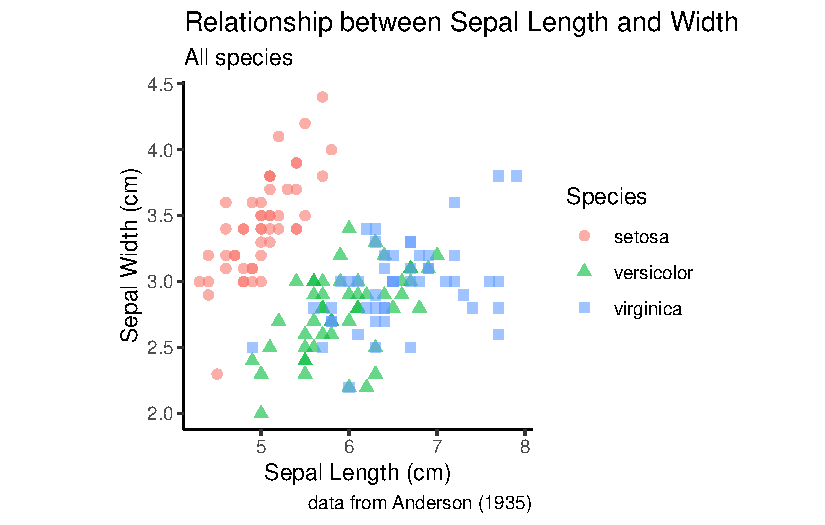
\includegraphics{_main_files/figure-latex/unnamed-chunk-2-1.pdf}
In fact, we don't need to supply random values at all. This could be a completely empty raster if we omit the \texttt{rnorm} argument altogether.

\begin{Shaded}
\begin{Highlighting}[]
\CommentTok{\#Generate 10000 random values in a 10x10 matrix}
\NormalTok{noValues}\OtherTok{\textless{}{-}}\FunctionTok{matrix}\NormalTok{(}\AttributeTok{nrow=}\DecValTok{100}\NormalTok{,}\AttributeTok{ncol=}\DecValTok{100}\NormalTok{)}

\CommentTok{\#Turn matrix into SpatRaster object}
\NormalTok{emptyRaster}\OtherTok{\textless{}{-}}\FunctionTok{rast}\NormalTok{(noValues)}

\CommentTok{\#Plot raster}
\FunctionTok{plot}\NormalTok{(emptyRaster)}
\end{Highlighting}
\end{Shaded}

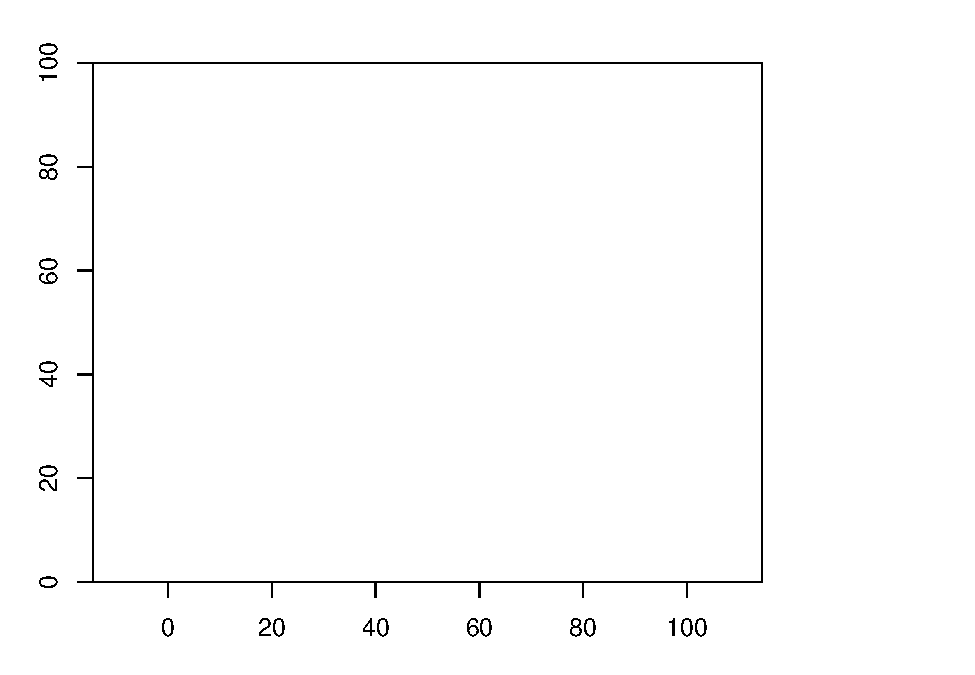
\includegraphics{_main_files/figure-latex/unnamed-chunk-3-1.pdf}

Values in a raster, empty or otherwise, can be added or modified in a number of ways. One way we can plug in values to our raster is with the \texttt{values} function. In this case, we'll sort some random values before they get added by wrapping the \texttt{rnorm} call in the\texttt{sort} function.

\begin{Shaded}
\begin{Highlighting}[]
\CommentTok{\#Add values to the empty raster}
\FunctionTok{values}\NormalTok{(emptyRaster)}\OtherTok{\textless{}{-}}\FunctionTok{sort}\NormalTok{(}\FunctionTok{runif}\NormalTok{(}\DecValTok{10000}\NormalTok{,}\DecValTok{0}\NormalTok{,}\DecValTok{1}\NormalTok{))}
\CommentTok{\#Plot the now not{-}so{-}empty raster}
\FunctionTok{plot}\NormalTok{(emptyRaster)}
\end{Highlighting}
\end{Shaded}

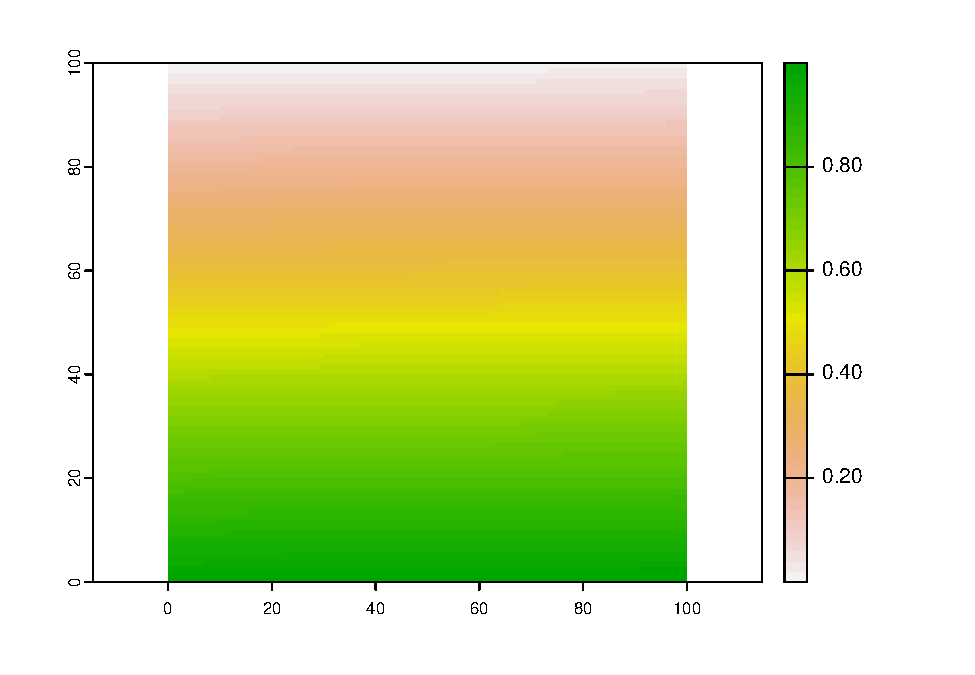
\includegraphics{_main_files/figure-latex/unnamed-chunk-4-1.pdf}

\hypertarget{non-numeric-rasters}{%
\section{Non-numeric rasters}\label{non-numeric-rasters}}

Since rasters typically represent continuous data, it makes sense that they often contain numeric values. However, this needn't always be the case. Here we'll make a raster of different landcover types. First, let's create a vector with some landcover types:

\begin{Shaded}
\begin{Highlighting}[]
\CommentTok{\#Land cover types}
\NormalTok{lctypes}\OtherTok{\textless{}{-}}\FunctionTok{c}\NormalTok{(}\StringTok{"grassland"}\NormalTok{,}\StringTok{"forest"}\NormalTok{,}\StringTok{"shrubland"}\NormalTok{)}
\end{Highlighting}
\end{Shaded}

Next, we'll generate a sample of 100 landcovers with the \texttt{sample} function:

\begin{Shaded}
\begin{Highlighting}[]
\CommentTok{\#Sample landcover types}
\NormalTok{landcover}\OtherTok{\textless{}{-}}\FunctionTok{sample}\NormalTok{(lctypes,}\DecValTok{100}\NormalTok{,}\AttributeTok{replace=}\ConstantTok{TRUE}\NormalTok{)}
\CommentTok{\#Look at the sample}
\NormalTok{landcover}
\end{Highlighting}
\end{Shaded}

\begin{verbatim}
##   [1] "shrubland" "grassland" "shrubland" "grassland" "shrubland" "shrubland"
##   [7] "forest"    "forest"    "grassland" "grassland" "shrubland" "grassland"
##  [13] "shrubland" "grassland" "grassland" "shrubland" "grassland" "forest"   
##  [19] "shrubland" "grassland" "shrubland" "shrubland" "shrubland" "forest"   
##  [25] "shrubland" "grassland" "shrubland" "grassland" "forest"    "grassland"
##  [31] "grassland" "grassland" "shrubland" "grassland" "forest"    "forest"   
##  [37] "forest"    "forest"    "grassland" "shrubland" "grassland" "forest"   
##  [43] "forest"    "grassland" "shrubland" "grassland" "shrubland" "grassland"
##  [49] "grassland" "grassland" "forest"    "forest"    "grassland" "shrubland"
##  [55] "forest"    "grassland" "shrubland" "forest"    "grassland" "forest"   
##  [61] "shrubland" "shrubland" "forest"    "forest"    "grassland" "grassland"
##  [67] "shrubland" "shrubland" "forest"    "forest"    "shrubland" "forest"   
##  [73] "forest"    "shrubland" "forest"    "shrubland" "grassland" "forest"   
##  [79] "shrubland" "grassland" "forest"    "forest"    "grassland" "shrubland"
##  [85] "shrubland" "grassland" "shrubland" "forest"    "grassland" "forest"   
##  [91] "shrubland" "forest"    "forest"    "forest"    "shrubland" "grassland"
##  [97] "forest"    "grassland" "shrubland" "grassland"
\end{verbatim}

Now we can create a 10x10 raster of landcover types using \texttt{rast}:

\begin{Shaded}
\begin{Highlighting}[]
\CommentTok{\#Make landcover raster}
\NormalTok{lcRaster}\OtherTok{\textless{}{-}}\FunctionTok{rast}\NormalTok{(}\AttributeTok{ncols=}\DecValTok{10}\NormalTok{,}\AttributeTok{nrows=}\DecValTok{10}\NormalTok{,}\AttributeTok{resolution =} \DecValTok{1}\NormalTok{, }\AttributeTok{xmin =} \DecValTok{0}\NormalTok{, }\AttributeTok{xmax =} \DecValTok{10}\NormalTok{, }\AttributeTok{ymin =} \DecValTok{0}\NormalTok{, }\AttributeTok{ymax =} \DecValTok{10}\NormalTok{,}\AttributeTok{vals=}\NormalTok{landcover)}
\CommentTok{\#Plot landcover raster}
\FunctionTok{plot}\NormalTok{(lcRaster)}
\end{Highlighting}
\end{Shaded}

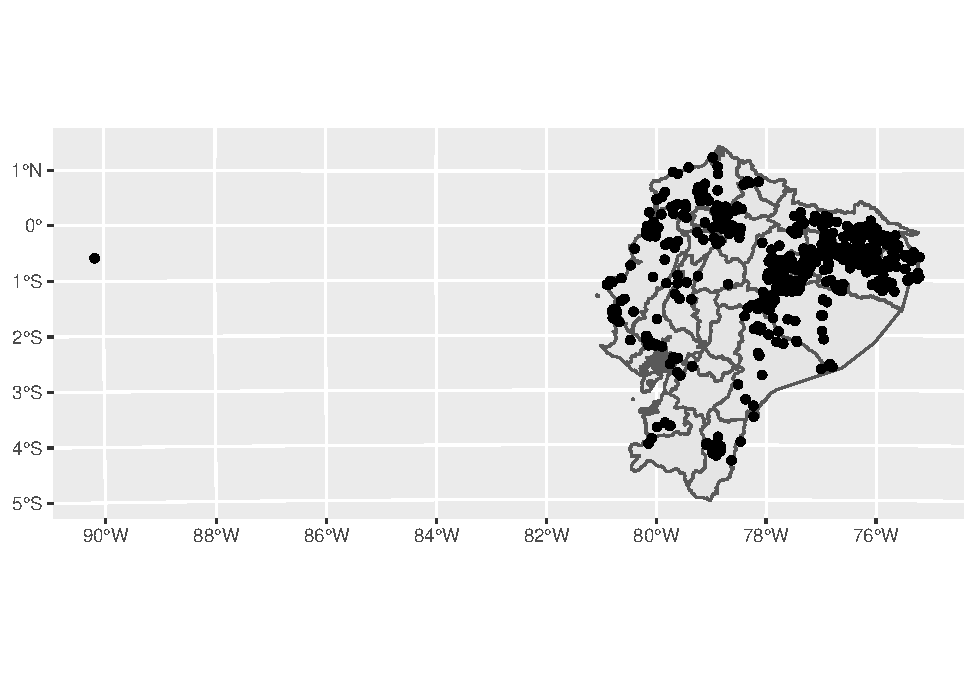
\includegraphics{_main_files/figure-latex/unnamed-chunk-7-1.pdf}
Nice! Finally, we can also make rasters that have boolean, or TRUE/FALSE, values. Here, we'll make a raster that shows whether a cell in our landcover raster is forested or not.

\begin{Shaded}
\begin{Highlighting}[]
\CommentTok{\#Make a true/false raster of forest cells}
\NormalTok{forestMask}\OtherTok{\textless{}{-}}\NormalTok{lcRaster}\SpecialCharTok{==}\StringTok{"forest"}
\CommentTok{\#Take a look}
\NormalTok{forestMask}
\end{Highlighting}
\end{Shaded}

\begin{verbatim}
## class       : SpatRaster 
## dimensions  : 10, 10, 1  (nrow, ncol, nlyr)
## resolution  : 1, 1  (x, y)
## extent      : 0, 10, 0, 10  (xmin, xmax, ymin, ymax)
## coord. ref. : lon/lat WGS 84 
## source      : memory 
## name        : lyr.1 
## min value   : FALSE 
## max value   :  TRUE
\end{verbatim}

The values of this new raster are now only true or false. We can take a look at this in a plot.

\begin{Shaded}
\begin{Highlighting}[]
\CommentTok{\#Plot the forest true/false}
\FunctionTok{plot}\NormalTok{(forestMask)}
\end{Highlighting}
\end{Shaded}

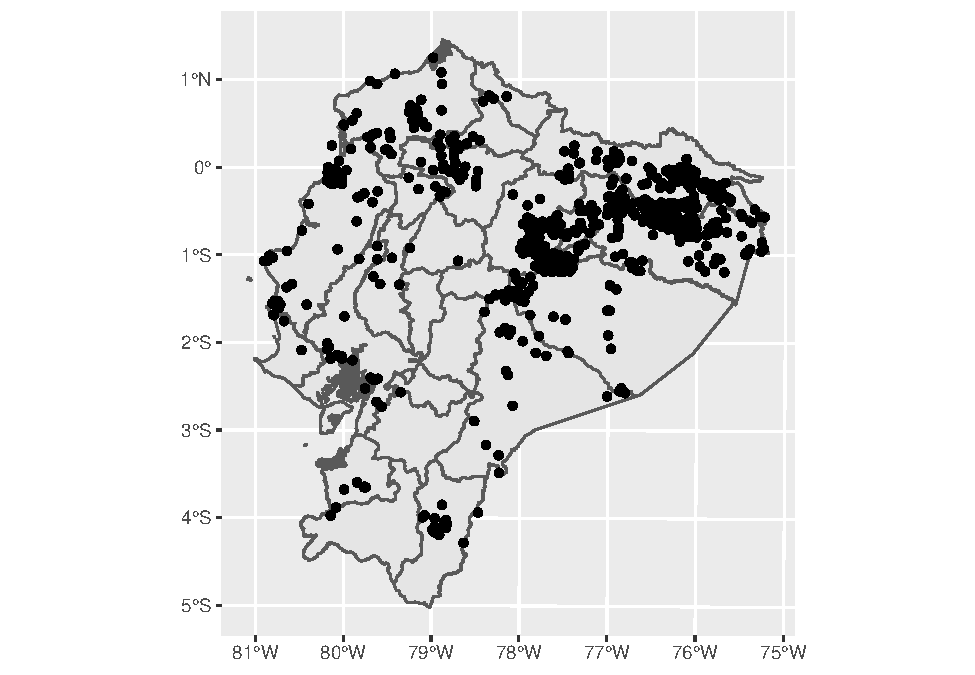
\includegraphics{_main_files/figure-latex/unnamed-chunk-9-1.pdf}

Boolean rasters can be especially useful as \emph{masks}, or a layer that is used to include or omit certain cells from an operation. We'll look at how these work later on.

\hypertarget{try-it-yourself}{%
\section{Try it yourself!}\label{try-it-yourself}}

Try and do the following

\begin{itemize}
\tightlist
\item
  Generate a 20x20 matrix of 400 random uniform values between 0 and 100
\item
  Turn this into a raster and plot it
\item
  Use this to create a boolean raster of values greater than 80.
\item
  Create a multilayer raster from the two rasters you've made
\end{itemize}

\hypertarget{working-with-raster-data}{%
\chapter{Working with raster data}\label{working-with-raster-data}}

\hypertarget{reading-in-a-raster-dataset}{%
\section{Reading in a raster dataset}\label{reading-in-a-raster-dataset}}

Let's use the \texttt{rast} function to read in an elevation from the area around Ngorongoro Crater and Olduvai Gorge in Tanzania.

\begin{Shaded}
\begin{Highlighting}[]
\CommentTok{\#Import the ngoronogoro.tif raster }
\NormalTok{ngorongoro}\OtherTok{\textless{}{-}}\FunctionTok{rast}\NormalTok{(}\StringTok{"ngorongoro.tif"}\NormalTok{)}
\end{Highlighting}
\end{Shaded}

This dataset comes from \href{https://www.gebco.net/}{General Bathymetric Chart of the Oceans (GEBCO)}, a bathymetric product from the British Oceanographic Data Centre that also serves as a decent source for terrestrial elevation data.

We can take a look at the attributes of this dataset just by calling its name.

\begin{Shaded}
\begin{Highlighting}[]
\CommentTok{\#Examine the data attributes}
\NormalTok{ngorongoro}
\end{Highlighting}
\end{Shaded}

\begin{verbatim}
## class       : SpatRaster 
## dimensions  : 240, 240, 1  (nrow, ncol, nlyr)
## resolution  : 0.004166667, 0.004166667  (x, y)
## extent      : 35, 36, -3.5, -2.5  (xmin, xmax, ymin, ymax)
## coord. ref. : lon/lat WGS 84 (EPSG:4326) 
## source      : ngorongoro.tif 
## name        : ngorongoro
\end{verbatim}

Here we can get a lot of helpful information. Going line by line:
* the class a \texttt{terra} SpatRaster
* the dimensions of the raster are 240x240 with one layer
* the resolution is 0.004166667 (this may seem a bit arbitrary, but this is the decimal degree equivalent of 15 seconds, or 0.25 minutes, of latitude/longitude; .
* the extent of the raster is 35 to 36 degrees longitude, -3.5
* the coordinate reference system is WGS 84 (EPSG:4326), or longitude/latitude

A couple of things you might notice. First, the latitude values for the extent are negative values. This is because we are using decimal degrees rather than degrees:minues:seconds to refer to geographic coordinates, and decimal degrees below the equator go from 0 to -90.

Second, the resolution of 0.004166667 may seem a little arbitrary. This value the decimal degree equivalent of 0.25 minutes, of latitude/longitude. You can read more about these two systems \href{https://gisgeography.com/decimal-degrees-dd-minutes-seconds-dms/}{here}.

\hypertarget{extract-values-from-raster}{%
\section{Extract values from raster}\label{extract-values-from-raster}}

Rasters are gridded data representing a continuous dataset across space. We can interrogate this data by finding individual values, or summarizing these for some focal area or the entire dataset.

First, let's get some individual values out of this. First, let's find the minimum elevation of the dataset.

\begin{Shaded}
\begin{Highlighting}[]
\CommentTok{\#Get minimum value for the whole dataset}
\FunctionTok{global}\NormalTok{(ngorongoro,}\StringTok{"min"}\NormalTok{)}
\end{Highlighting}
\end{Shaded}

\begin{verbatim}
##            min
## ngorongoro 593
\end{verbatim}

And then the maximum elevation:

\begin{Shaded}
\begin{Highlighting}[]
\CommentTok{\#Get minimum value for the whole dataset}
\FunctionTok{global}\NormalTok{(ngorongoro,}\StringTok{"max"}\NormalTok{)}
\end{Highlighting}
\end{Shaded}

\begin{verbatim}
##             max
## ngorongoro 3582
\end{verbatim}

This gives a sense of the range of values, but it doesn't tell us much about they vary. One way we could characterize this would be to get the mean and standard deviation for all the elevation on the grid.

\begin{Shaded}
\begin{Highlighting}[]
\CommentTok{\#Get mean for the whole dataset}
\FunctionTok{global}\NormalTok{(ngorongoro,}\StringTok{"mean"}\NormalTok{)}
\end{Highlighting}
\end{Shaded}

\begin{verbatim}
##                mean
## ngorongoro 1640.887
\end{verbatim}

\begin{Shaded}
\begin{Highlighting}[]
\CommentTok{\#Get standard deviation for the whole dataset}
\FunctionTok{global}\NormalTok{(ngorongoro,}\StringTok{"sd"}\NormalTok{)}
\end{Highlighting}
\end{Shaded}

\begin{verbatim}
##                  sd
## ngorongoro 460.3775
\end{verbatim}

This shows an average of around 1641 meters a.s.l. and a standard deviation of around 460 meters. If we're interested in the shape of the distribution, we could plug the raster into a histogram and see how they are distributed.

\begin{Shaded}
\begin{Highlighting}[]
\CommentTok{\#histogram of raster values}
\FunctionTok{hist}\NormalTok{(ngorongoro)}
\end{Highlighting}
\end{Shaded}

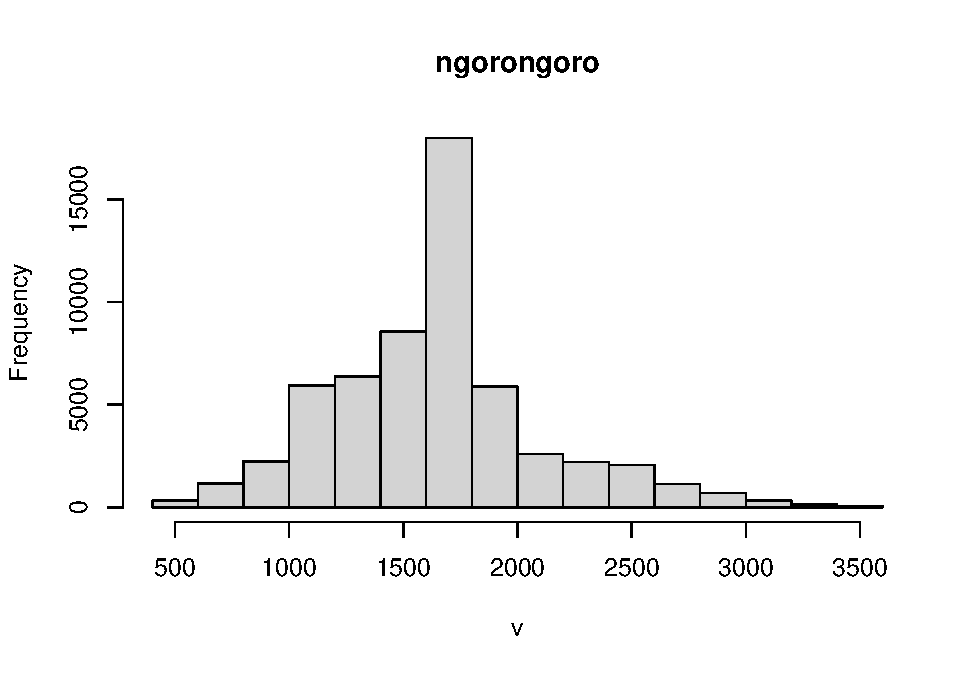
\includegraphics{_main_files/figure-latex/unnamed-chunk-15-1.pdf}
This tells us a fair bit more about how t However, the thing that makes geographic data interesting is that they not only vary, but co-vary with location.

We can see this by extracting a transect of elevation values. We'll do this by taking all the values in a row across the middle of the raster. Rows are numbered top to bottom; knowing that the raster is 240x240, the midde row is 120. Once we have that, we can turn it into a vector of values using the \texttt{\$} operator.

\begin{Shaded}
\begin{Highlighting}[]
\CommentTok{\#Get elevation across middle row}
\NormalTok{elevationTransect}\OtherTok{\textless{}{-}}\NormalTok{ngorongoro[}\DecValTok{120}\NormalTok{,]}
\CommentTok{\#Turn it into a vector}
\NormalTok{elevation}\OtherTok{\textless{}{-}}\NormalTok{elevationTransect}\SpecialCharTok{$}\NormalTok{ngorongoro}
\CommentTok{\#Show values}
\NormalTok{elevation}
\end{Highlighting}
\end{Shaded}

\begin{verbatim}
##   [1] 1589 1592 1617 1626 1629 1631 1632 1633 1632 1632 1631 1630 1628 1628 1628
##  [16] 1627 1626 1626 1626 1624 1623 1621 1618 1613 1607 1595 1588 1595 1585 1578
##  [31] 1581 1577 1576 1579 1595 1601 1599 1590 1588 1592 1598 1600 1621 1623 1619
##  [46] 1612 1607 1600 1591 1586 1581 1576 1571 1568 1564 1561 1558 1555 1551 1545
##  [61] 1538 1533 1530 1528 1526 1525 1522 1520 1518 1517 1510 1490 1474 1470 1461
##  [76] 1453 1461 1465 1461 1457 1454 1453 1449 1458 1460 1465 1453 1433 1458 1464
##  [91] 1464 1462 1451 1443 1438 1417 1384 1369 1364 1361 1360 1356 1344 1339 1320
## [106] 1313 1310 1307 1305 1303 1301 1299 1296 1293 1291 1290 1289 1296 1308 1321
## [121] 1338 1366 1404 1442 1487 1565 1637 1679 1715 1756 1826 1909 1993 2066 2114
## [136] 2172 2229 2304 2384 2432 2476 2546 2611 2662 2711 2744 2785 2868 2939 2988
## [151] 3054 3016 2927 2903 2897 2889 2898 2900 2900 2895 2889 2904 2990 2945 2817
## [166] 2683 2596 2550 2521 2505 2488 2472 2443 2425 2420 2417 2371 2313 2313 2315
## [181] 2318 2325 2336 2349 2366 2386 2406 2429 2452 2482 2513 2547 2577 2609 2639
## [196] 2638 2659 2714 2789 2798 2772 2739 2701 2678 2646 2623 2585 2561 2539 2520
## [211] 2495 2475 2454 2330 2154 2054 1984 1920 2027 2053 1970 1939 1890 1759 1601
## [226] 1382 1156 1026  991  968  946  917  901  890  881  871  863  855  849  843
\end{verbatim}

This is all the elevation in each cell of row 120. To visualize how this changes over space, we should also have the sequence of decimal degrees between 35 and 36 longitude in our raster. We can use \texttt{seq} to generate these.

\begin{Shaded}
\begin{Highlighting}[]
\CommentTok{\#Get a list of decimal degrees}
\NormalTok{degrees}\OtherTok{\textless{}{-}}\FunctionTok{seq}\NormalTok{(}\DecValTok{35}\NormalTok{,}\DecValTok{36}\NormalTok{,}\AttributeTok{length.out=}\DecValTok{240}\NormalTok{)}
\NormalTok{degrees}
\end{Highlighting}
\end{Shaded}

\begin{verbatim}
##   [1] 35.00000 35.00418 35.00837 35.01255 35.01674 35.02092 35.02510 35.02929
##   [9] 35.03347 35.03766 35.04184 35.04603 35.05021 35.05439 35.05858 35.06276
##  [17] 35.06695 35.07113 35.07531 35.07950 35.08368 35.08787 35.09205 35.09623
##  [25] 35.10042 35.10460 35.10879 35.11297 35.11715 35.12134 35.12552 35.12971
##  [33] 35.13389 35.13808 35.14226 35.14644 35.15063 35.15481 35.15900 35.16318
##  [41] 35.16736 35.17155 35.17573 35.17992 35.18410 35.18828 35.19247 35.19665
##  [49] 35.20084 35.20502 35.20921 35.21339 35.21757 35.22176 35.22594 35.23013
##  [57] 35.23431 35.23849 35.24268 35.24686 35.25105 35.25523 35.25941 35.26360
##  [65] 35.26778 35.27197 35.27615 35.28033 35.28452 35.28870 35.29289 35.29707
##  [73] 35.30126 35.30544 35.30962 35.31381 35.31799 35.32218 35.32636 35.33054
##  [81] 35.33473 35.33891 35.34310 35.34728 35.35146 35.35565 35.35983 35.36402
##  [89] 35.36820 35.37238 35.37657 35.38075 35.38494 35.38912 35.39331 35.39749
##  [97] 35.40167 35.40586 35.41004 35.41423 35.41841 35.42259 35.42678 35.43096
## [105] 35.43515 35.43933 35.44351 35.44770 35.45188 35.45607 35.46025 35.46444
## [113] 35.46862 35.47280 35.47699 35.48117 35.48536 35.48954 35.49372 35.49791
## [121] 35.50209 35.50628 35.51046 35.51464 35.51883 35.52301 35.52720 35.53138
## [129] 35.53556 35.53975 35.54393 35.54812 35.55230 35.55649 35.56067 35.56485
## [137] 35.56904 35.57322 35.57741 35.58159 35.58577 35.58996 35.59414 35.59833
## [145] 35.60251 35.60669 35.61088 35.61506 35.61925 35.62343 35.62762 35.63180
## [153] 35.63598 35.64017 35.64435 35.64854 35.65272 35.65690 35.66109 35.66527
## [161] 35.66946 35.67364 35.67782 35.68201 35.68619 35.69038 35.69456 35.69874
## [169] 35.70293 35.70711 35.71130 35.71548 35.71967 35.72385 35.72803 35.73222
## [177] 35.73640 35.74059 35.74477 35.74895 35.75314 35.75732 35.76151 35.76569
## [185] 35.76987 35.77406 35.77824 35.78243 35.78661 35.79079 35.79498 35.79916
## [193] 35.80335 35.80753 35.81172 35.81590 35.82008 35.82427 35.82845 35.83264
## [201] 35.83682 35.84100 35.84519 35.84937 35.85356 35.85774 35.86192 35.86611
## [209] 35.87029 35.87448 35.87866 35.88285 35.88703 35.89121 35.89540 35.89958
## [217] 35.90377 35.90795 35.91213 35.91632 35.92050 35.92469 35.92887 35.93305
## [225] 35.93724 35.94142 35.94561 35.94979 35.95397 35.95816 35.96234 35.96653
## [233] 35.97071 35.97490 35.97908 35.98326 35.98745 35.99163 35.99582 36.00000
\end{verbatim}

Now we can plot these together to see how elevation changes across space!

\begin{Shaded}
\begin{Highlighting}[]
\FunctionTok{plot}\NormalTok{(degrees,elevation,}\AttributeTok{type=}\StringTok{"l"}\NormalTok{)}
\end{Highlighting}
\end{Shaded}

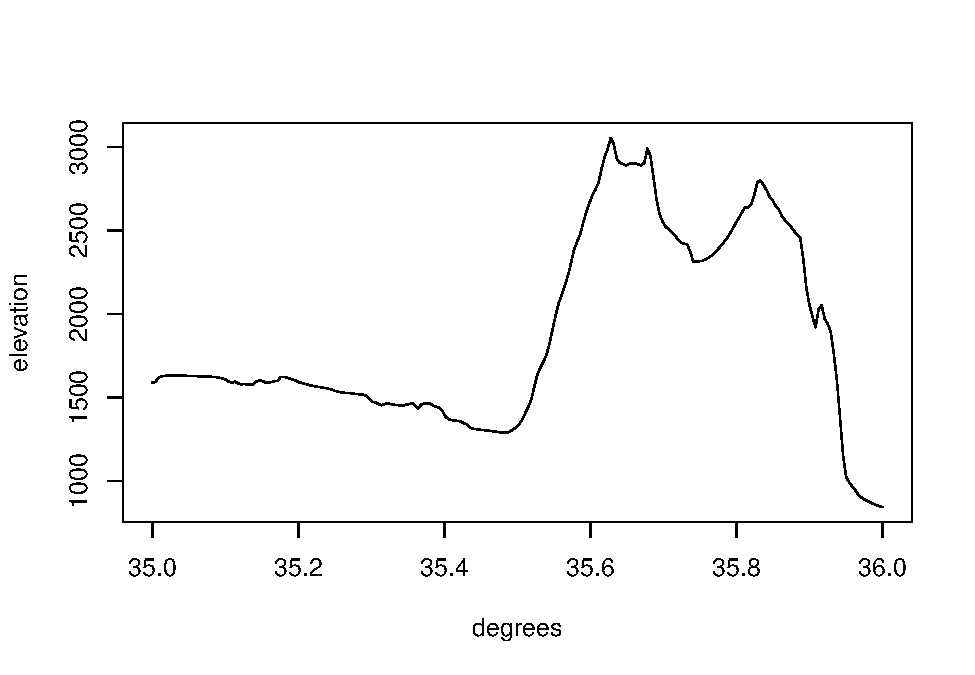
\includegraphics{_main_files/figure-latex/unnamed-chunk-18-1.pdf}

What we can see from this plot is that there is a plain in the west that sits around 1600 meters a.s.l. (close to our mean value). Going east from there is a steep elevation gain followed by some peaks, and then a steep drop off levels below 1000 meters a.s.l.

We can also see this when we plot the data.

\begin{Shaded}
\begin{Highlighting}[]
\CommentTok{\#Plot raster}
\FunctionTok{plot}\NormalTok{(ngorongoro)}
\end{Highlighting}
\end{Shaded}

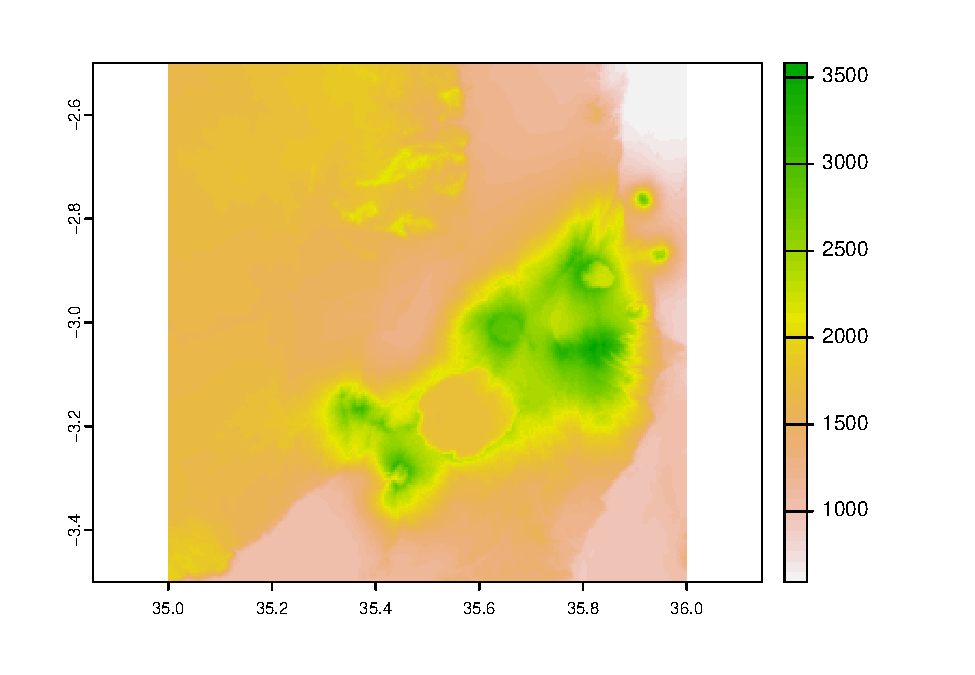
\includegraphics{_main_files/figure-latex/unnamed-chunk-19-1.pdf}

\hypertarget{multilayer-rasters}{%
\chapter{Multilayer rasters}\label{multilayer-rasters}}

\hypertarget{reading-in-a-multilayer-raster-dataset}{%
\section{Reading in a multilayer raster dataset}\label{reading-in-a-multilayer-raster-dataset}}

This time we'll look at some satellite imagery from the eastern shore of Lake Turkana, taken in January 2020.

\begin{Shaded}
\begin{Highlighting}[]
\CommentTok{\#Import the northTurkana.tif raster }
\NormalTok{eastTurkana}\OtherTok{\textless{}{-}}\FunctionTok{rast}\NormalTok{(}\StringTok{"eastTurkana.tif"}\NormalTok{)}
\end{Highlighting}
\end{Shaded}

Once again, let's look at the attributes:

\begin{Shaded}
\begin{Highlighting}[]
\CommentTok{\#Examine the data attributes}
\NormalTok{eastTurkana}
\end{Highlighting}
\end{Shaded}

\begin{verbatim}
## class       : SpatRaster 
## dimensions  : 1380, 1166, 4  (nrow, ncol, nlyr)
## resolution  : 3, 3  (x, y)
## extent      : 193059, 196557, 477168, 481308  (xmin, xmax, ymin, ymax)
## coord. ref. : WGS 84 / UTM zone 37N (EPSG:32637) 
## source      : eastTurkana.tif 
## names       : blue, green, red, nir
\end{verbatim}

This is similar to the last dataset except for one important detail: there are 4 layers in this dataset. In the \texttt{names} area, we can see these are \emph{blue}, \emph{green}, \emph{red}, and \emph{nir} (which stands for ``near-infrared). We can look at each of these with \texttt{plot}.

\hypertarget{plotting}{%
\section{Plotting}\label{plotting}}

\begin{Shaded}
\begin{Highlighting}[]
\FunctionTok{plot}\NormalTok{(eastTurkana)}
\end{Highlighting}
\end{Shaded}

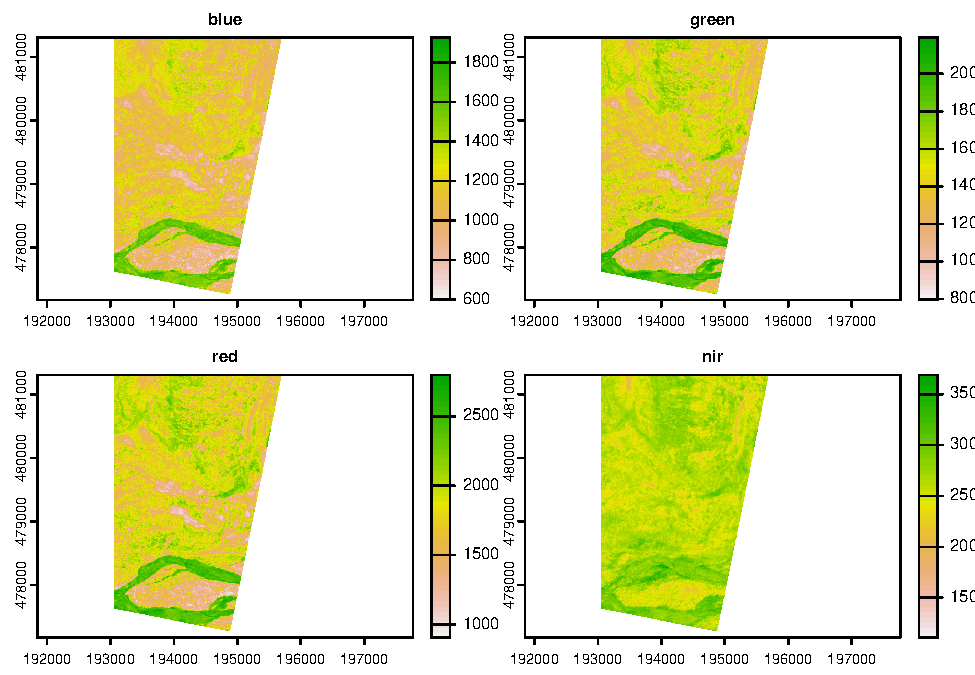
\includegraphics{_main_files/figure-latex/unnamed-chunk-22-1.pdf}

The names of the layers are different colors, but these are sensor values of surface reflectance in these different spectra, so R just plots them all on a similar scale. If we wanted to just plot one layer, we can use double brackets \texttt{{[}{[}{]}{]}} and call it by its number in the layer order.

\begin{Shaded}
\begin{Highlighting}[]
\CommentTok{\#Plot just the red}
\FunctionTok{plot}\NormalTok{(eastTurkana[[}\DecValTok{3}\NormalTok{]])}
\end{Highlighting}
\end{Shaded}

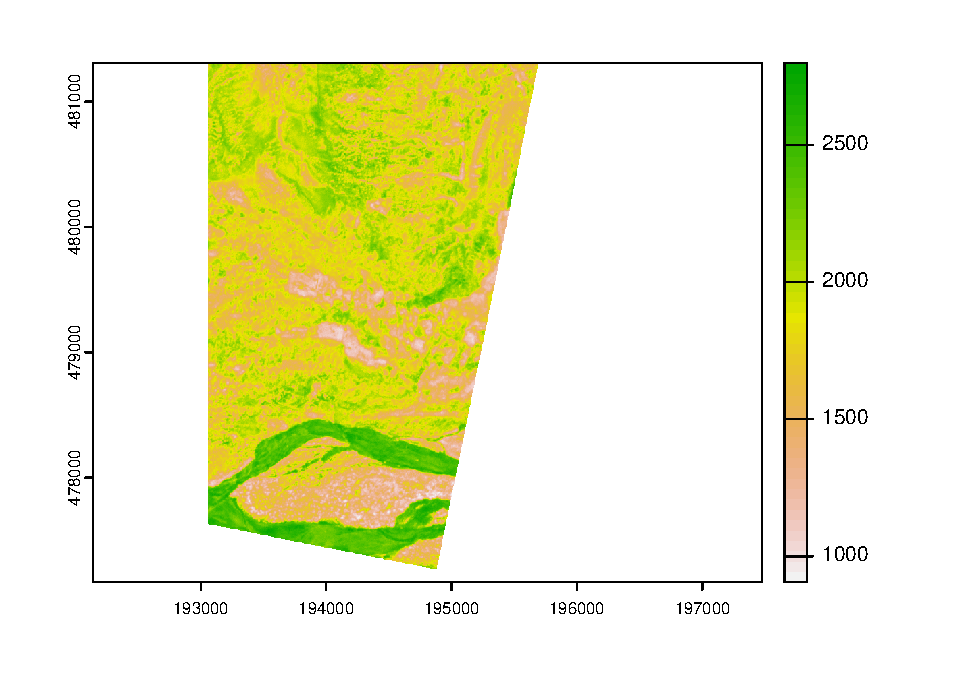
\includegraphics{_main_files/figure-latex/unnamed-chunk-23-1.pdf}

Or we can use single brackets \texttt{{[}{]}} and call it by it's name in quotation marks.

\begin{Shaded}
\begin{Highlighting}[]
\CommentTok{\#Plot just the red another way}
\FunctionTok{plot}\NormalTok{(eastTurkana[}\StringTok{\textquotesingle{}red\textquotesingle{}}\NormalTok{])}
\end{Highlighting}
\end{Shaded}

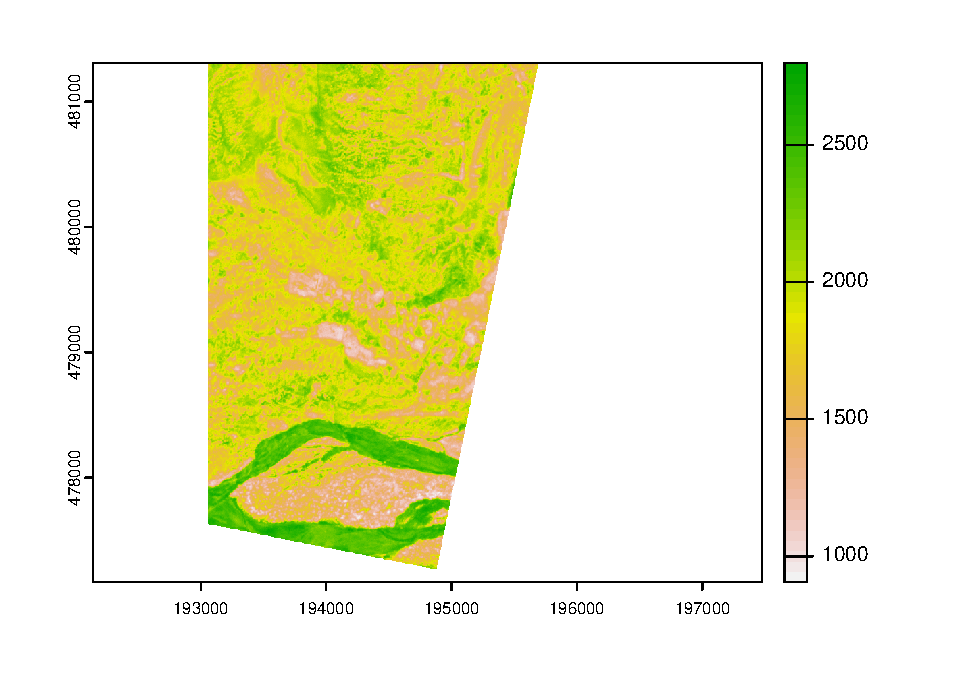
\includegraphics{_main_files/figure-latex/unnamed-chunk-24-1.pdf}

If plotting a ``red'' layer without using the color red is bothering you as much as it bothers me, we'll need to look at using \texttt{RColorBrewer}, specifically the \texttt{brewer.pal} function. This takes two arguments: a number and a `palette'. In this case, we're going to use the ``Reds'' palette.

\begin{Shaded}
\begin{Highlighting}[]
\CommentTok{\#Plot reds as reds}
\FunctionTok{plot}\NormalTok{(eastTurkana[}\StringTok{\textquotesingle{}red\textquotesingle{}}\NormalTok{],}\AttributeTok{col=}\FunctionTok{brewer.pal}\NormalTok{(}\DecValTok{9}\NormalTok{,}\StringTok{"Reds"}\NormalTok{))}
\end{Highlighting}
\end{Shaded}

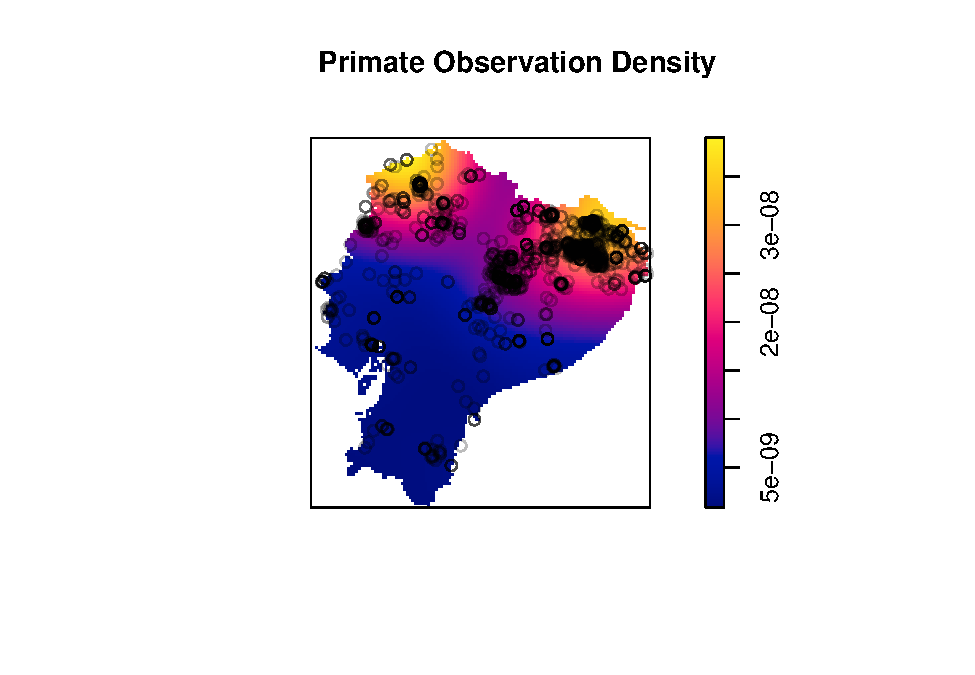
\includegraphics{_main_files/figure-latex/unnamed-chunk-25-1.pdf}

You can read more about the different approaches to color, including the RColorBrewer palettes, at \href{https://bootstrappers.umassmed.edu/bootstrappers-courses/pastCourses/rCourse_2016-04/Additional_Resources/Rcolorstyle.html}{this page}

\hypertarget{raster-algebra}{%
\section{Raster algebra}\label{raster-algebra}}

These sensor reflectance values, called ``digital numbers'', are highly exaggerated. To convert them to reasonable reflectance values, we need to divide them by 10000.

\begin{Shaded}
\begin{Highlighting}[]
\CommentTok{\#Divide raster values by 10000}
\NormalTok{eastTurkana2}\OtherTok{\textless{}{-}}\NormalTok{eastTurkana}\SpecialCharTok{/}\DecValTok{10000}
\CommentTok{\#}
\FunctionTok{plot}\NormalTok{(eastTurkana2)}
\end{Highlighting}
\end{Shaded}

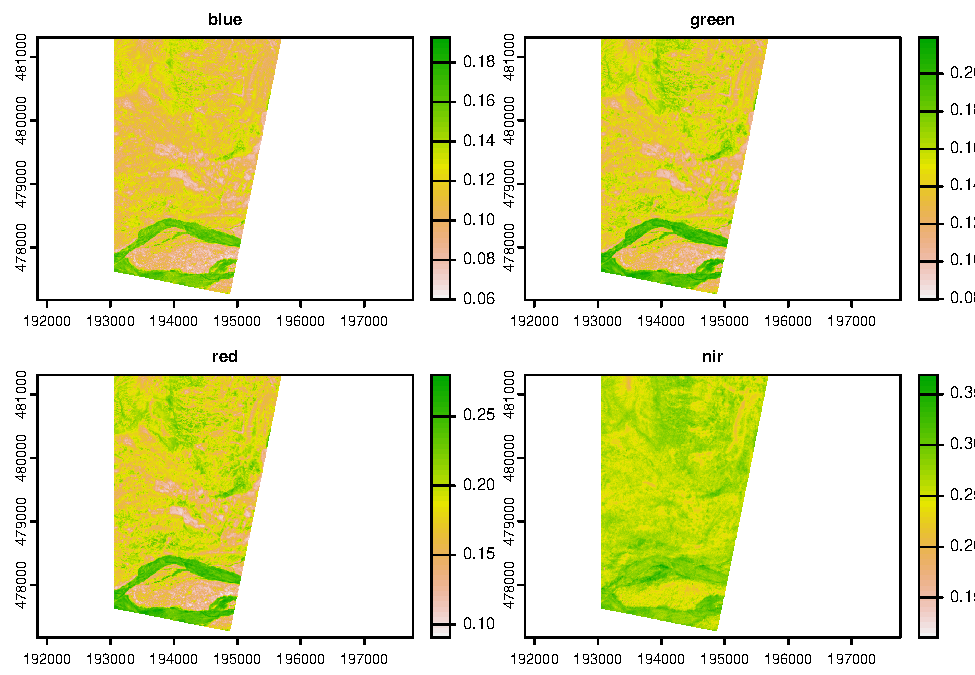
\includegraphics{_main_files/figure-latex/unnamed-chunk-26-1.pdf}

We can also do raster math using the different layers of this dataset. For example, let's say we were interested in calculating the \href{https://gisgeography.com/ndvi-normalized-difference-vegetation-index/}{Normalized Difference Vegetation Index}: a measure of vegetation greenness that is used as an indicator of vegetation cover. The equation for this is \emph{NDVI = (NIR --- RED)/(NIR + RED)}.

Two make things simple, we'll get rasters: one for red, and one for near infrared.

\begin{Shaded}
\begin{Highlighting}[]
\NormalTok{red}\OtherTok{\textless{}{-}}\NormalTok{eastTurkana2[}\StringTok{\textquotesingle{}red\textquotesingle{}}\NormalTok{]}
\NormalTok{nir}\OtherTok{\textless{}{-}}\NormalTok{eastTurkana2[}\StringTok{\textquotesingle{}nir\textquotesingle{}}\NormalTok{]}

\FunctionTok{plot}\NormalTok{(red)}
\end{Highlighting}
\end{Shaded}

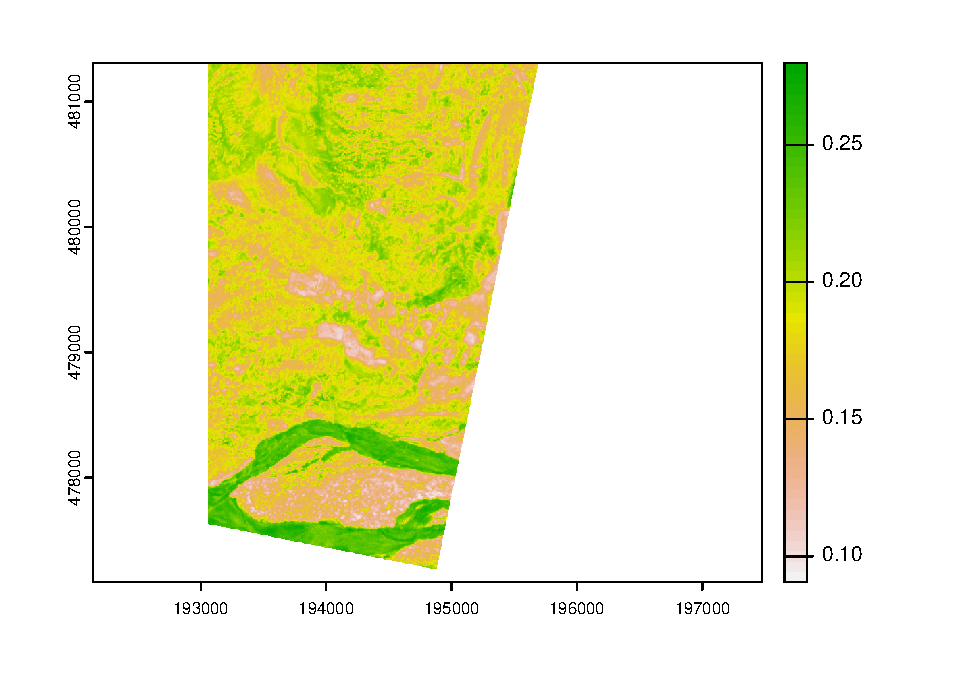
\includegraphics{_main_files/figure-latex/unnamed-chunk-27-1.pdf}

\begin{Shaded}
\begin{Highlighting}[]
\FunctionTok{plot}\NormalTok{(nir)}
\end{Highlighting}
\end{Shaded}

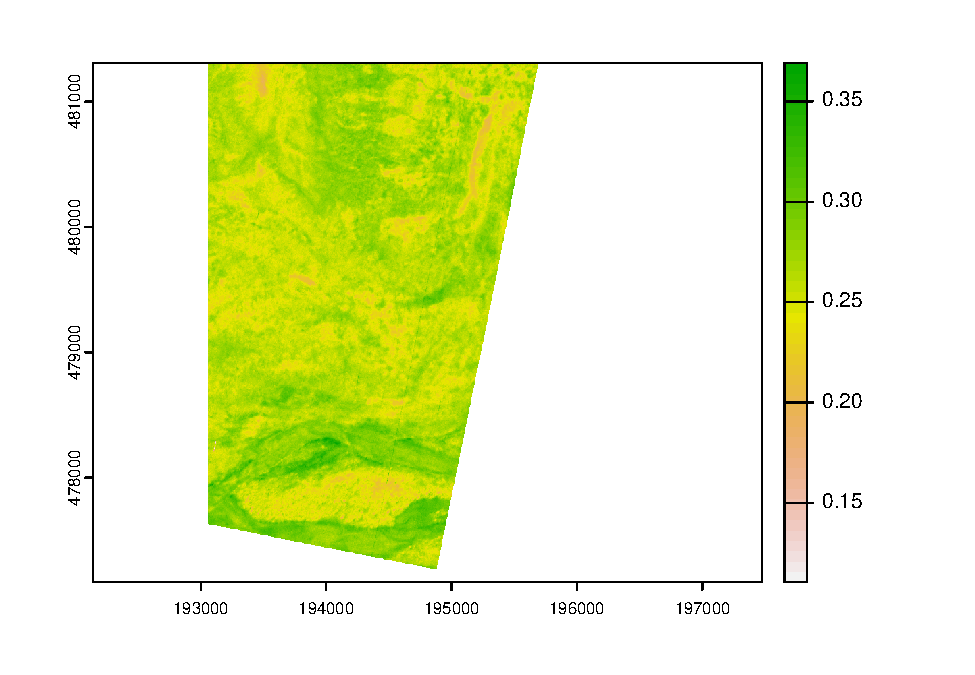
\includegraphics{_main_files/figure-latex/unnamed-chunk-27-2.pdf}

Now, we can insert them into the equation for NDVI:

\begin{Shaded}
\begin{Highlighting}[]
\NormalTok{ndvi}\OtherTok{\textless{}{-}}\NormalTok{(nir}\SpecialCharTok{{-}}\NormalTok{red)}\SpecialCharTok{/}\NormalTok{(nir}\SpecialCharTok{+}\NormalTok{red)}
\FunctionTok{plot}\NormalTok{(ndvi)}
\end{Highlighting}
\end{Shaded}

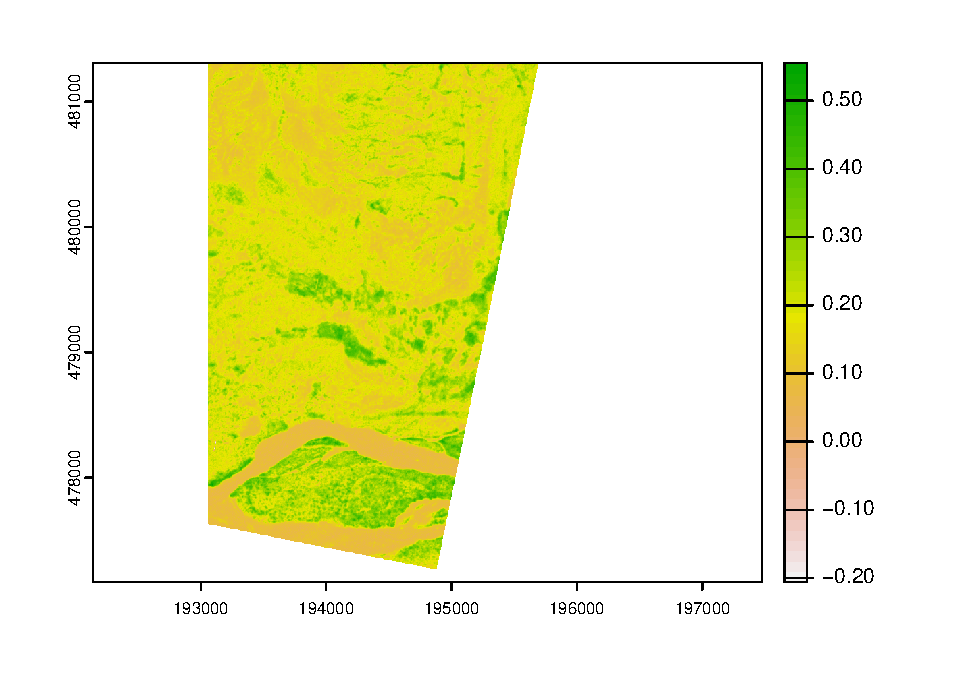
\includegraphics{_main_files/figure-latex/unnamed-chunk-28-1.pdf}

Generally speaking, the higher the value, the greener the vegetation. Values below 0 are bare rock or water. In this image of a semi-arid landscape, greener values tend to be along stream lines and in areas that hold water.

\hypertarget{try-it-yourself-1}{%
\section{Try it yourself!}\label{try-it-yourself-1}}

Use the eastTurkana dataset to do the following:

\begin{itemize}
\tightlist
\item
  Plot the green and blue bands using an appropriate color palette.
\item
  Another measurement like NDVI is the Normalized Difference Water Index. The formula for this is \emph{NDWI = (GREEN -- NIR) / (GREEN + NIR)}. Create subsets for the green and near infrared layers and then create this index. Plot it. Where are the highest values? Are any values over 0.3 (the minimum threshold for water surface)?
\item
  What is the coordinate reference system of the eastTurkana dataset?
\end{itemize}

\hypertarget{bring-it-all-together}{%
\chapter{Bring it all together!}\label{bring-it-all-together}}

Try to write code to do the following on your own:

\begin{itemize}
\tightlist
\item
  Load the turkanaRain raster dataset
\item
  Create a subset of the last 50 months in the dataset
\item
  Use \texttt{global} to get the mean values for this subset and then create a histogram from these values (hint: you may need to use the \texttt{\$} operator)
\item
  Create a raster that is the sum of the last 10 years (120 months) of rainfall data
\item
  Plot this raster in a blue palette
\end{itemize}

  \bibliography{book.bib,packages.bib}

\end{document}
